%=========================================================================
% Example Using the Automatic LaTeX Build System
%=========================================================================

\newcommand{\hackdocumentclass}{\documentclass}
\hackdocumentclass[sigconf]{acmart}
\usepackage{cbxutils}

% Automatix LaTeX build system modules

\usepackage{svg}
\usepackage{py}

% Ensure letter paper

\pdfpagewidth=8.5in
\pdfpageheight=11in

\begin{document}

%-------------------------------------------------------------------------
% Front Matter
%-------------------------------------------------------------------------

\copyrightyear{XXXX}
\acmYear{XXXX}
\setcopyright{acmcopyright}
\acmConference{CONF-01}{Month 1--2, XXXX}{Ithaca, NY, USA}
\acmPrice{15.00}
\acmDOI{XX.XXXX/XXXX.XXXX}
\acmISBN{XXX-X-XXXX-XXXX-X/XX/XX}

\title
[%
  Example Using the ALBS
]{%
  Example Using the Automatic LaTeX Build System
}

\author{%
  Christopher Batten
}

\affiliation{
  \vspace{0.07in}
  \institution{%
    School of Electrical and Computer Engineering,
    Cornell University, Ithaca, NY%
  }
}

\email{%
  cbatten@cornell.edu%
  \vspace{0.05in}
}

% List the first author for headers

\renewcommand{\shortauthors}{C. Batten}

% The code below should be generated by the tool at
% http://dl.acm.org/ccs.cfm
% Please copy and paste the code instead of the example below.

\begin{CCSXML}
\end{CCSXML}

\ccsdesc[500]{Computer Systems}

\keywords{computer systems}

%=========================================================================
% Abstract
%=========================================================================

\begin{abstract}
  \lipsum[1]
\end{abstract}



\maketitle

%-------------------------------------------------------------------------
% Body
%-------------------------------------------------------------------------

%=========================================================================
% Introduction
%=========================================================================

\section{Introduction}
\label{sec-intro}

\lipsum[1-3]


%=========================================================================
% Motivation
%=========================================================================

\section{Motivation}
\label{sec-motivation}

%=========================================================================
% fig-example.tex
%=========================================================================
% Place figure code in a separate file to make body text in the section
% files easier to read, and to simplify moving around figures.

\begin{figure}

  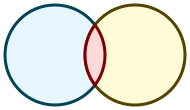
\includegraphics[width=0.5\tw]{example.svg.pdf}

  \caption{\textbf{Example Figure Title --} \normalfont{Descriptive text
      which usually also describes any acronyms used in the figure.}}
  \label{fig-example}

\end{figure}



\lipsum[1-5]


%=========================================================================
% Approach
%=========================================================================

\section{Approach}
\label{sec-approach}

%=========================================================================
% fig-plot-example
%=========================================================================

\begin{figure}[t]

  \includegraphics[width=\cw]{plot-example.py.pdf}

  \caption{\textbf{Example Figure Title --} \normalfont{Descriptive text
      which usually also describes any acronyms used in the plot.}}
  \label{fig-plot-example}

\end{figure}



\lipsum[1-5]


%=========================================================================
% Methodology
%=========================================================================

\section{Methodology}
\label{sec-methodology}

\lipsum[1-5]


%=========================================================================
% Evaluation
%=========================================================================

\section{Evaluation}
\label{sec-evaluation}

\lipsum[1-5]


%=========================================================================
% Related Work
%=========================================================================

\section{Related Work}
\label{sec-related}

\lipsum[1]~\cite{jiang-mamba-dac2018, bukreyev-dcs-tcasi2018,
  kim-lta-micro2014, srinath-xloops-micro2014}

\lipsum[2-3]


%=========================================================================
% Conclustions
%=========================================================================

\section{Conclusions}
\label{sec-conclusions}

\lipsum[1]



%-------------------------------------------------------------------------
% Back Matter
%-------------------------------------------------------------------------

\begin{acks}
  This work was supported in part by ...
\end{acks}

%\clearpage
\bibliographystyle{acmart}
\balance
\bibliography{cbatten}

\end{document}

